\providecommand{\UseMathForPositioningText}{}
\documentclass[11pt,a4paper]{article}

\usepackage{geometry}
\geometry{top=2.5cm,bottom=2.5cm,left=2.5cm,right=2.5cm}
\usepackage{graphicx}
\usepackage{setspace}
\usepackage{tikz}
\usetikzlibrary{calc,arrows.meta,positioning,fit,shapes.geometric}
\usepackage{eso-pic}
\usepackage{titlesec}
\usepackage{float}
\usepackage{amsmath}
\usepackage{amssymb}
\usepackage{booktabs}
\usepackage{array}
\usepackage{caption}
\usepackage{tocloft}
\usepackage{xcolor}
\usepackage{hyperref}
\usepackage{listings}
\usepackage{enumitem}
\usepackage{longtable}
\usepackage{tabularx}
\usepackage{pifont}
\usepackage{xepersian}

\IfFontExistsTF{XB Niloofar}
  {\settextfont{XB Niloofar}}
  {\settextfont{Noto Naskh Arabic}}

\IfFontExistsTF{DejaVu Sans}
  {\setlatintextfont{DejaVu Sans}}
  {}

\IfFontExistsTF{DejaVu Sans Mono}
  {\setmonofont{DejaVu Sans Mono}}
  {}

\titleformat{\section}{\fontsize{18pt}{22pt}\bfseries}{\thesection}{1em}{}
\titleformat{\subsection}{\fontsize{15pt}{19pt}\bfseries}{\thesubsection}{1em}{}
\titleformat{\subsubsection}{\fontsize{13pt}{17pt}\bfseries}{\thesubsubsection}{1em}{}
\renewcommand{\cftsecleader}{\cftdotfill{\cftdotsep}}

\setstretch{1.25}
\setlength{\parindent}{1.2cm}
\setlength{\parskip}{0.35em}
\setlength{\emergencystretch}{2em}
\setlength{\footnotesep}{0.5cm}
\renewcommand{\arraystretch}{1.35}

\newcommand{\enfoot}[1]{\LTRfootnote{#1}}
\newcommand{\code}[1]{\lr{\texttt{\detokenize{#1}}}}
\newcommand{\filename}[1]{\lr{\texttt{\detokenize{#1}}}}
\newcommand{\passmark}{\textcolor{black}{\ding{51}}}
\renewcommand{\labelitemi}{\(\bullet\)}
\renewcommand{\lstlistingname}{کد}

\lstdefinestyle{verilogstyle}{
  language=Verilog,
  basicstyle=\ttfamily\small,
  numbers=left,
  numberstyle=\tiny,
  stepnumber=1,
  numbersep=8pt,
  frame=single,
  rulecolor=\color{black!45},
  backgroundcolor=\color{black!3},
  keywordstyle=\color{blue!55!black}\bfseries,
  commentstyle=\color{green!35!black},
  stringstyle=\color{red!55!black},
  showstringspaces=false,
  breaklines=true,
  breakatwhitespace=false,
  tabsize=4,
  columns=fullflexible,
  keepspaces=true,
  captionpos=b
}
\lstset{style=verilogstyle}

\newcommand{\reportimage}[2][0.96\textwidth]{%
  \IfFileExists{#2}%
    {\includegraphics[width=#1]{#2}}%
    {\fbox{\parbox[c][5.2cm][c]{0.88\textwidth}{\centering\textbf{محلّ قرارگیری تصویر}\\[0.35cm]\lr{\texttt{#2}}}}}%
}

\begin{document}

\AddToShipoutPictureBG{
  \begin{tikzpicture}[remember picture,overlay]
    \node[
      draw,
      line width=2.5pt,
      minimum width=\paperwidth-2cm,
      minimum height=\paperheight-2cm,
      inner sep=0pt
    ] at (current page.center) {};
    \node[
      draw,
      line width=1pt,
      minimum width=\paperwidth-2.3cm,
      minimum height=\paperheight-2.3cm,
      inner sep=0pt
    ] at (current page.center) {};
  \end{tikzpicture}
}

\begin{titlepage}
  \centering
  \vspace*{0.1cm}

  \IfFileExists{images/logo.png}
    {
\includegraphics[width=2.9cm]{images/logo.png}}
    {\fbox{\parbox[c][2.6cm][c]{2.6cm}{\centering\lr{images/logo.png}}}}
  \\[0.35cm]
  {\fontsize{13pt}{17pt}\selectfont دانشگاه صنعتی شریف}\\[0.1cm]
  {\fontsize{13pt}{17pt}\selectfont دانشکده مهندسی کامپیوتر}

  \vspace{0.75cm}
  {\fontsize{15pt}{19pt}\bfseries گزارش کار آزمایش دهم}

  \vspace{0.7cm}
  {\fontsize{11.5pt}{15pt}\selectfont عنوان:}\\[0.3cm]
  {\fontsize{19pt}{25pt}\bfseries پیاده‌سازی و توسعهٔ یک پردازندهٔ ساده}

  \vspace{0.75cm}
  {\fontsize{11.5pt}{15pt}\selectfont نام درس}\\[0.25cm]
  {\fontsize{13.5pt}{17pt}\bfseries آزمایشگاه طراحی سامانه‌های رقمی}

  \vspace{0.6cm}
  {\fontsize{11.5pt}{15pt}\selectfont تابستان ۱۴۰۵}

  \vspace{0.6cm}
  {\fontsize{11.5pt}{15pt}\selectfont استاد}\\[0.2cm]
  {\fontsize{13pt}{17pt}\bfseries دکتر اجلالی}

  \vspace{0.45cm}
  {\fontsize{11.5pt}{15pt}\selectfont دستیار استاد}\\[0.2cm]
  {\fontsize{13pt}{17pt}\bfseries علی اثنی عشری}

  \vspace{0.55cm}
  {\fontsize{11.5pt}{15pt}\selectfont گروه ۲\par}

  \vspace{0.25cm}
  {\fontsize{13pt}{17pt}\bfseries
  علی سلطانی ـ ۴۰۳۱۰۶۰۹۲\\[0.12cm]
  یگانه کربلایی ـ ۴۰۳۱۰۶۵۲۷\\[0.12cm]
  محمدمهدی مرادی ـ ۴۰۳۱۰۶۶۸۱\par}

  \vfill
\end{titlepage}

\newpage
\tableofcontents
\newpage

\section{هدف آزمایش}

هدف این آزمایش، توسعه و پیاده‌سازی یک پردازنده با معماری پشته‌ای\enfoot{Stack Architecture} است که دارای یک پشته با هشت ثبات هشت‌بیتی و حافظه‌ای با ۲۵۶ خانۀ هشت‌بیتی است. هشت خانۀ انتهایی فضای نشانی، یعنی \code{F8} تا \code{FF}، برای ورودی و خروجی نگاشت‌شده در حافظه\enfoot{Memory-Mapped I/O} در نظر گرفته می‌شوند و ارتباط پردازنده با کلیدها، چراغ‌ها و نمایشگرهای هفت‌قسمتی\enfoot{Seven-Segment Display} فقط از طریق همین نشانی‌ها انجام می‌شود.

پردازندۀ پایه با سه دستور \code{SWAP}، \code{SHL} و \code{CMP} توسعه داده می‌شود و در نتیجه مجموعۀ نهایی شامل ۱۱ دستور است. برای پشتیبانی از این سه دستور، مسیر داده\enfoot{Datapath} و واحد کنترل\enfoot{Control Unit} توسعه یافته‌اند. در ادامه، با استفاده از همین پردازنده، برنامه‌ای در سطح کد ماشین\enfoot{Machine Code} نوشته شده است که مقدار هشت‌بیتی \(X\) را دریافت کرده و تابع چندبخشی خواسته‌شده را محاسبه می‌کند.

تابع مورد نظر برابر است با
\[
Y=
\begin{cases}
3X+5, & 0\le X<32,\\
2X+20, & 32\le X<64,\\
X-40, & 64\le X\le 127.
\end{cases}
\]
تشخیص بازۀ ورودی با دستور \code{CMP} و پرش‌های شرطی انجام می‌شود. همچنین برای محاسبۀ \(2X\) از \code{SHL} و برای \(3X\) از رابطۀ \(3X=X+2X\) استفاده شده است؛ بنابراین در بخش قابل سنتز طراحی هیچ عملگر ضرب مستقیمی برای پیاده‌سازی تابع وجود ندارد.

\section{مشخّصات معماری و قرارداد پشته}

\subsection{ساختار کلّی پردازنده}

پشته شامل هشت ثبات هشت‌بیتی است و اشاره‌گر پشته به نخستین خانۀ خالی اشاره می‌کند. مقدار بالاترین عنصر پشته با \(A\) و عنصر دوّم از بالا با \(B\) نمایش داده می‌شود. در پیاده‌سازی حاضر:
\[
A=\text{stack[SP-1]},\qquad
B=\text{stack[SP-2]}.
\]
در دستورهای دو عملوندی \code{ADD} و \code{SUB} دو عنصر بالا با یک نتیجه جایگزین می‌شوند. مطابق تعریف تفصیلی دستورها، تفریق به‌صورت
\[
B-A
\]
انجام می‌شود و همین تفاضل در دستور \code{CMP} نیز برای به‌روزرسانی پرچم‌ها به‌کار می‌رود.

پردازنده دارای دو پرچم \code{S} و \code{Z} است. \code{Z} در صورت صفر بودن نتیجۀ محاسبه یک می‌شود و \code{S} برابر بیت شمارهٔ هفت نتیجۀ هشت‌بیتی است. تنها دستورهای \code{ADD}، \code{SUB} و \code{CMP} مجاز به تغییر این دو پرچم هستند. تمام محاسبات علامت‌دار و مبتنی بر نمایش متمّم دو انجام می‌شوند.

\subsection{مجموعۀ دستورها}

کد عملیاتی\enfoot{Opcode} هر دستور در چهار بیت کم‌ارزش ثبات دستور قرار می‌گیرد. در دستورهای پرش، شمارندۀ برنامه\enfoot{Program Counter} مقصد اجرای بعدی را نگهداری می‌کند. جدول \ref{tab:isa} مجموعۀ کامل ۱۱ دستور را نشان می‌دهد.

\begin{table}[H]
\centering
\small
\begin{tabularx}{\textwidth}{>{\centering\arraybackslash}p{2.0cm}
                            >{\centering\arraybackslash}p{2.1cm}
                            X}
\toprule
\textbf{دستور} & \textbf{کد عملیاتی} & \textbf{عملکرد} \\
\midrule
\lr{\texttt{PUSHC C}} & \lr{\texttt{0000}} & قرار دادن ثابت هشت‌بیتی \(C\) روی پشته \\
\lr{\texttt{PUSH M}}  & \lr{\texttt{0001}} & خواندن خانۀ حافظه یا درگاه ورودی \(M\) و قرار دادن آن روی پشته \\
\lr{\texttt{POP M}}   & \lr{\texttt{0010}} & حذف عنصر بالا و نوشتن آن در حافظه یا درگاه خروجی \(M\) \\
\lr{\texttt{JUMP}}    & \lr{\texttt{0011}} & حذف نشانی بالای پشته و قرار دادن آن در شمارندۀ برنامه \\
\lr{\texttt{JZ}}      & \lr{\texttt{0100}} & حذف نشانی پرش و پرش در صورت \code{Z=1} \\
\lr{\texttt{JS}}      & \lr{\texttt{0101}} & حذف نشانی پرش و پرش در صورت \code{S=1} \\
\lr{\texttt{ADD}}     & \lr{\texttt{0110}} & جایگزینی \(A\) و \(B\) با \(A+B\) و به‌روزرسانی \code{S,Z} \\
\lr{\texttt{SUB}}     & \lr{\texttt{0111}} & جایگزینی \(A\) و \(B\) با \(B-A\) و به‌روزرسانی \code{S,Z} \\
\lr{\texttt{SWAP}}    & \lr{\texttt{1000}} & جابه‌جایی دو عنصر بالای پشته بدون تغییر پرچم‌ها \\
\lr{\texttt{SHL}}     & \lr{\texttt{1001}} & انتقال یک‌بیتی عنصر بالای پشته به چپ بدون تغییر پرچم‌ها \\
\lr{\texttt{CMP}}     & \lr{\texttt{1010}} & محاسبۀ موقّت \(B-A\)، بدون تغییر پشته، و به‌روزرسانی \code{S,Z} \\
\bottomrule
\end{tabularx}
\caption{مجموعۀ دستورهای پردازندهٔ توسعه‌یافته}
\label{tab:isa}
\end{table}

کدهای \code{1011} تا \code{1111} رزروشده‌اند و در این آزمایش استفاده نشده‌اند.

\subsection{نمودار بلوکی پردازندهٔ توسعه‌یافته}

شکل \ref{fig:block-diagram} نمودار بلوکی پردازنده را نشان می‌دهد. حافظه و واحد ورودی و خروجی خارج از هسته قرار دارند و از طریق چهار سیگنال نشانی، دادهٔ خواندنی، دادهٔ نوشتنی و فعّال‌ساز نوشتن با پردازنده ارتباط برقرار می‌کنند.

\begin{figure}[H]
  \centering
  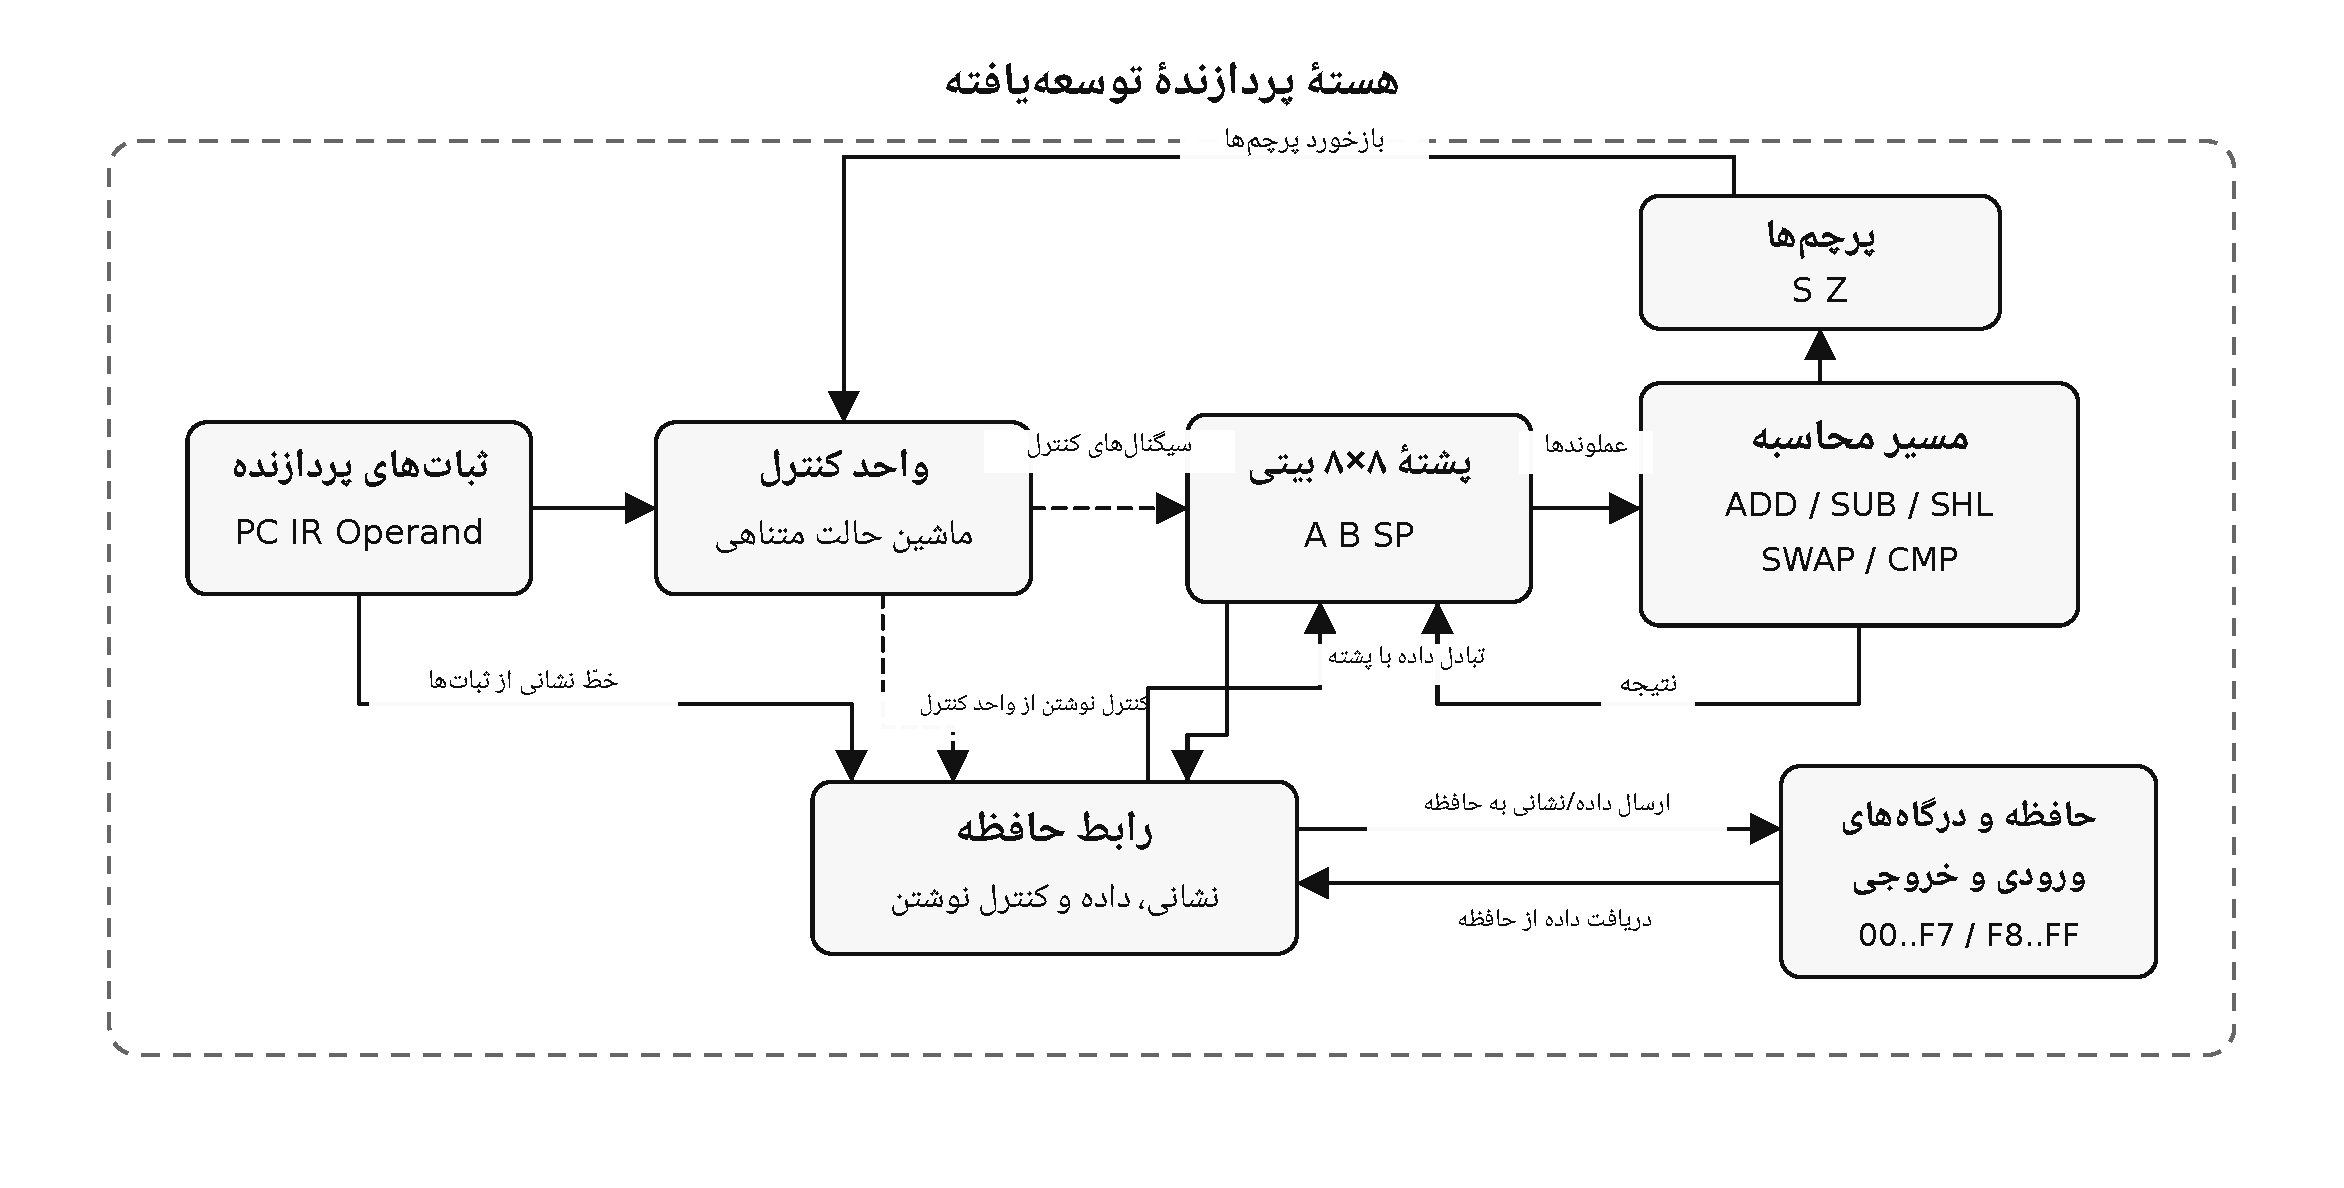
\includegraphics[width=0.94\textwidth]{images/processor_block_diagram.pdf}
  \caption{نمودار بلوکی پردازندهٔ توسعه‌یافته}
  \label{fig:block-diagram}
\end{figure}

\section{توسعهٔ مسیر داده برای سه دستور جدید}

\subsection{دستور \lr{SWAP}}

برای اجرای \code{SWAP} لازم است هر دو عنصر بالای پشته به‌طور هم‌زمان در دسترس باشند. در حالت اجرای این دستور، محتوای خانۀ \code{SP-1} با محتوای \code{SP-2} جابه‌جا می‌شود. اشاره‌گر پشته تغییر نمی‌کند و هیچ‌یک از پرچم‌ها نیز به‌روزرسانی نمی‌شوند. استفاده از انتساب‌های غیرمسدودکننده در منطق ترتیبی باعث می‌شود دو مقدار قدیمی به‌صورت صحیح با یکدیگر مبادله شوند.

\subsection{دستور \lr{SHL}}

برای \code{SHL} یک مسیر انتقال یک‌بیتی به چپ روی عنصر بالای پشته اضافه شده است:
\[
\text{Top}\leftarrow \text{Top}\ll 1.
\]
بیت صفر نتیجۀ جدید صفر می‌شود و بیت شمارهٔ هفت قبلی حذف می‌گردد. نتیجۀ هشت‌بیتی در همان خانۀ بالای پشته ذخیره می‌شود؛ بنابراین عمق پشته ثابت می‌ماند. مطابق صورت آزمایش، این دستور پرچم‌های \code{S} و \code{Z} را تغییر نمی‌دهد.

\subsection{دستور \lr{CMP}}

دستور \code{CMP} از همان مسیر تفریق استفاده می‌کند، امّا نتیجه را در پشته نمی‌نویسد. مقدار موقّت
\[
T=B-A
\]
محاسبه می‌شود و فقط پرچم‌ها از آن ساخته می‌شوند:
\[
Z=(T=0),\qquad S=T_7.
\]
ترتیب، عمق و محتوای پشته پس از اجرای \code{CMP} بدون تغییر باقی می‌ماند. همین ویژگی اجازه می‌دهد دو مقدار برای مقایسه روی پشته قرار گیرند، پرچم‌ها تعیین شوند و سپس دو عملوند با دو دستور \code{POP} پاک شوند.

\subsection{جدول ریزعملیات دستورهای جدید}

\begin{table}[H]
\centering
\small
\begin{tabularx}{\textwidth}{>{\centering\arraybackslash}p{2.0cm}
                            X
                            >{\centering\arraybackslash}p{2.2cm}
                            >{\centering\arraybackslash}p{2.5cm}}
\toprule
\textbf{دستور} & \textbf{ریزعملیات} & \textbf{تغییر \code{SP}} & \textbf{تغییر پرچم‌ها} \\
\midrule
\lr{\texttt{SWAP}} &
\(\text{stack[SP-1]}\leftarrow B,\;
  \text{stack[SP-2]}\leftarrow A\) &
بدون تغییر & بدون تغییر \\
\lr{\texttt{SHL}} &
\(\text{stack[SP-1]}\leftarrow A\ll1\) &
بدون تغییر & بدون تغییر \\
\lr{\texttt{CMP}} &
\(T\leftarrow B-A,\;
 Z\leftarrow(T=0),\;
 S\leftarrow T_7\) &
بدون تغییر & \code{S,Z} \\
\bottomrule
\end{tabularx}
\caption{ریزعملیات سه دستور جدید}
\label{tab:microops}
\end{table}

\section{توسعهٔ واحد کنترل}

واحد کنترل به‌صورت ماشین حالت متناهی\enfoot{Finite State Machine} پیاده‌سازی شده است. روند عمومی اجرای دستور شامل حالت‌های \code{FETCH} و \code{DECODE} است. دستورهای دارای عملوند هشت‌بیتی، یعنی \code{PUSHC}، \code{PUSH} و \code{POP}، پیش از اجرا وارد حالت \code{FETCH_OPERAND} می‌شوند. برای سه دستور جدید نیز سه حالت اجرایی مستقل \code{STATE_SWAP}، \code{STATE_SHL} و \code{STATE_CMP} به واحد کنترل افزوده شده‌اند.

در \code{JUMP}، نشانی بالای پشته همیشه حذف و در شمارندۀ برنامه قرار می‌گیرد. در \code{JZ} و \code{JS} نیز نشانی پرش در هر دو حالت برقرار یا برقرارنبودن شرط از پشته حذف می‌شود؛ تنها نوشتن در \code{PC} وابسته به پرچم مربوط است. این رفتار باعث می‌شود پس از یک پرش شرطی ناموفّق نیز نشانی مقصد روی پشته باقی نماند.

\begin{figure}[H]
  \centering
  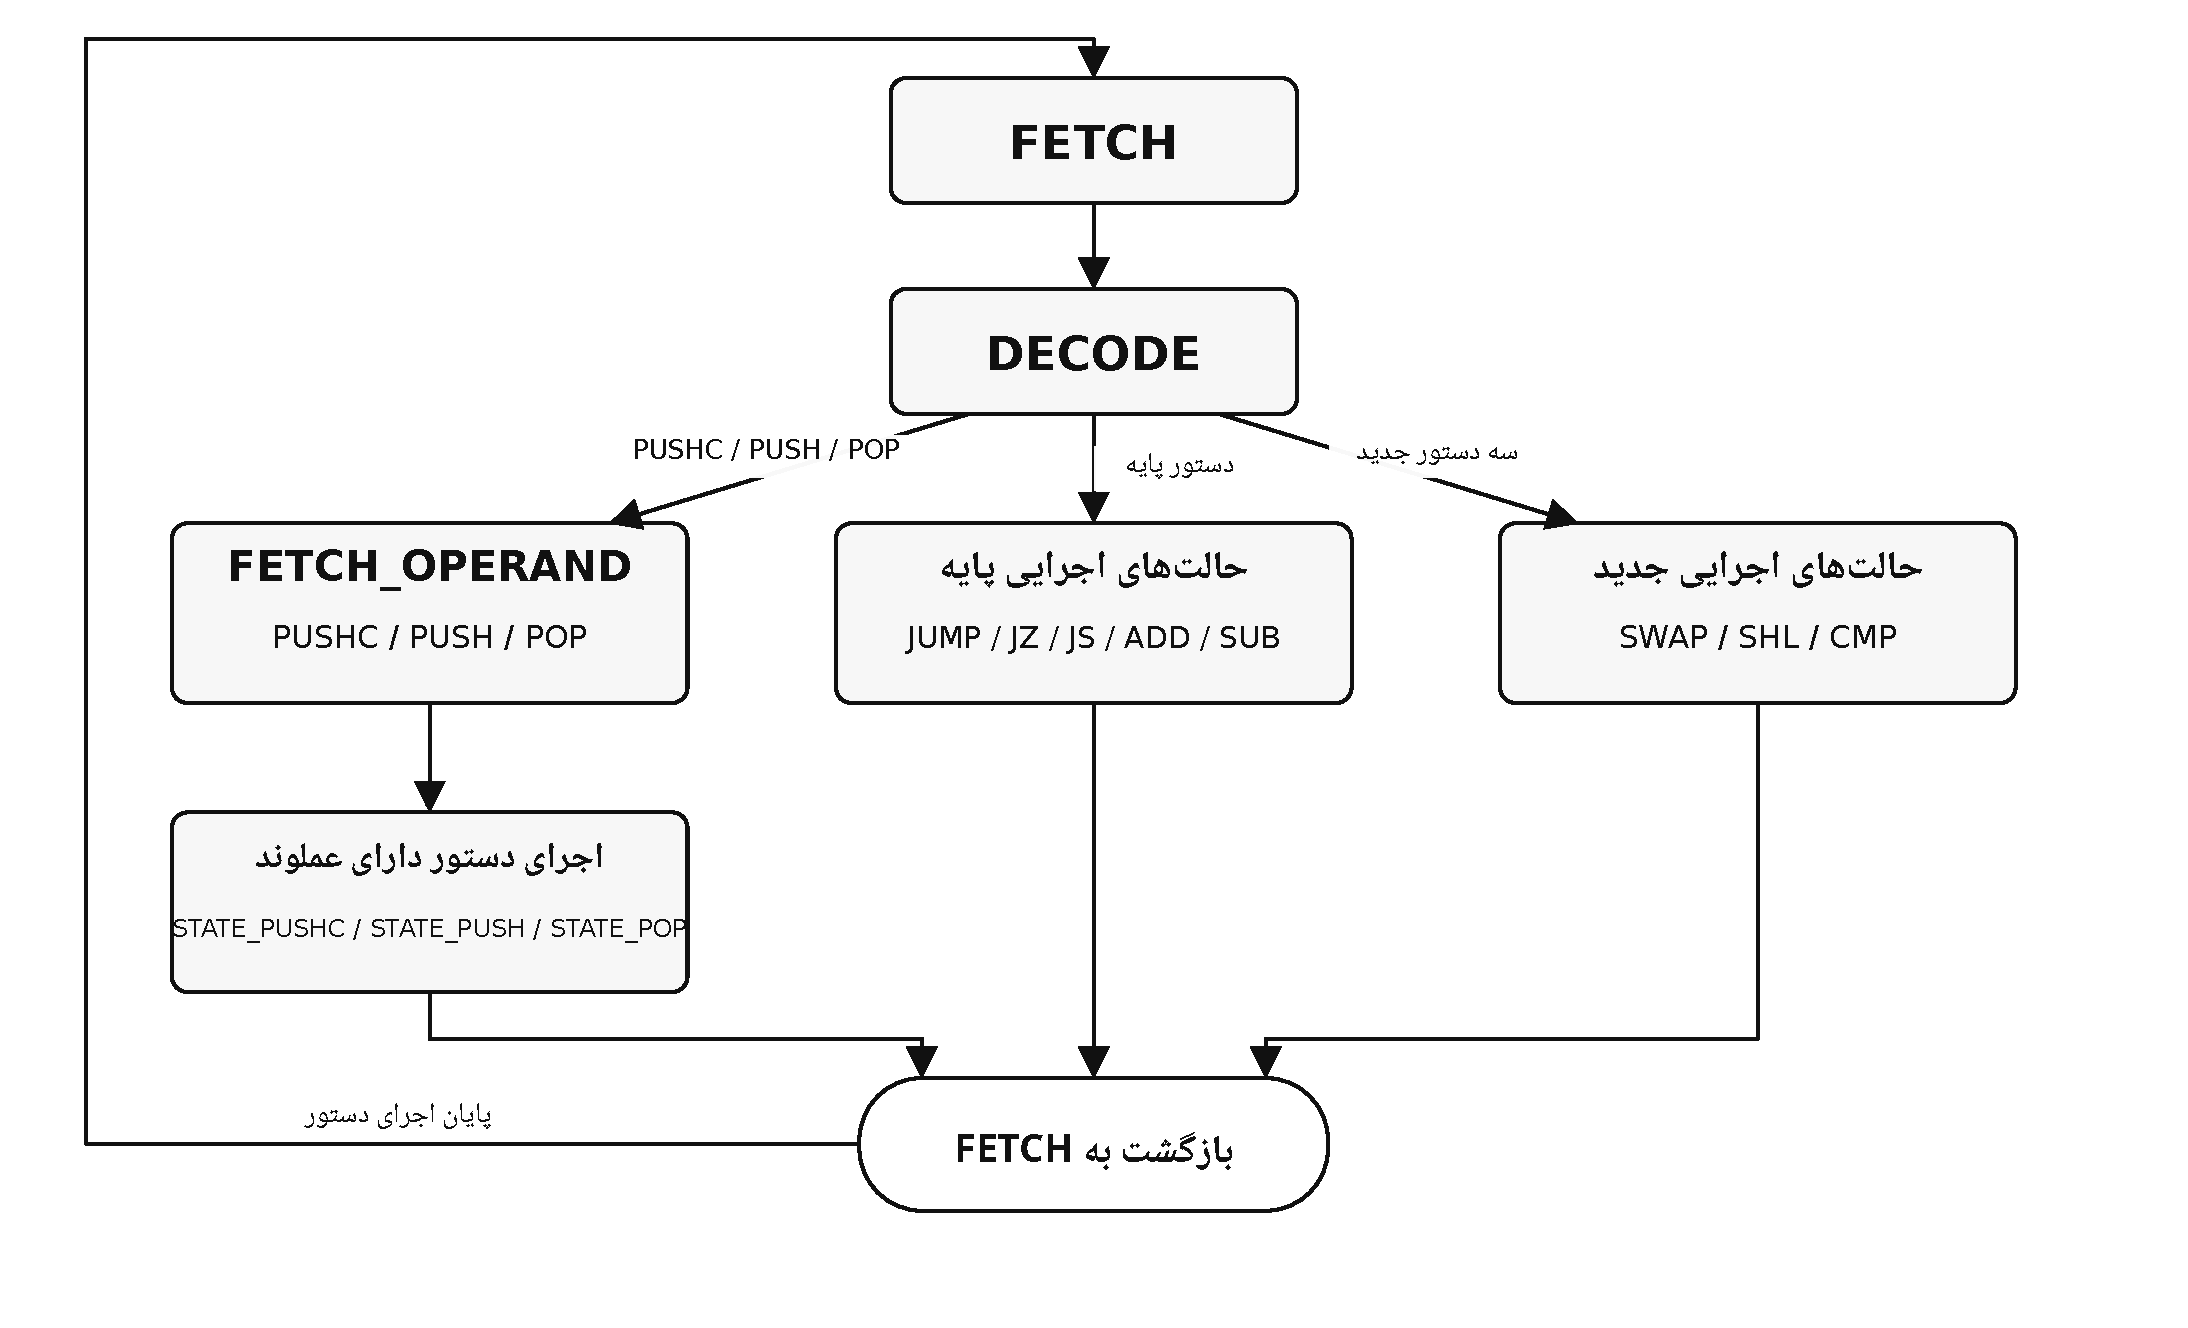
\includegraphics[width=0.92\textwidth]{images/control_unit_fsm.pdf}
  \caption{ساختار کلّی گذارهای واحد کنترل و افزوده‌شدن سه حالت جدید}
  \label{fig:control-fsm}
\end{figure}

\section{نگاشت حافظه و ورودی و خروجی}

حافظۀ عادی در بازۀ \code{00} تا \code{F7} قرار دارد و هشت نشانی انتهایی به درگاه‌های ورودی و خروجی اختصاص یافته‌اند. مقدار نهایی روی دو رقم در مبنای شانزده\enfoot{Hexadecimal} نمایش داده می‌شود. جدول \ref{tab:mmio} نگاشت مورد استفاده را نشان می‌دهد.

\begin{table}[H]
\centering
\begin{tabularx}{\textwidth}{>{\centering\arraybackslash}p{1.7cm}
                            >{\centering\arraybackslash}p{2.7cm}
                            X}
\toprule
\textbf{نشانی} & \textbf{نوع دسترسی} & \textbf{عملکرد} \\
\midrule
\lr{\texttt{F8}} & فقط‌خواندنی & ورودی هشت‌بیتی \(X\) از کلیدهای بورد \\
\lr{\texttt{F9}} & فقط‌نوشتنی & رقم کم‌ارزش خروجی در مبنای شانزده؛ فقط چهار بیت کم‌ارزش دادهٔ نوشته‌شده استفاده می‌شود \\
\lr{\texttt{FA}} & فقط‌نوشتنی & رقم پرارزش خروجی در مبنای شانزده؛ فقط چهار بیت کم‌ارزش دادهٔ نوشته‌شده استفاده می‌شود \\
\lr{\texttt{FB}} & فقط‌نوشتنی & بیت صفر، خروجی چراغ خطا \\
\lr{\texttt{FC}} & فقط‌نوشتنی & بیت صفر، خروجی چراغ پایان محاسبه \\
\lr{\texttt{FD--FF}} & رزروشده & در این آزمایش استفاده نمی‌شوند \\
\bottomrule
\end{tabularx}
\caption{نگاشت ورودی و خروجی در فضای نشانی}
\label{tab:mmio}
\end{table}

در حالت موفّق، ابتدا خطا صفر می‌شود، رقم کم‌ارزش در \code{F9} و رقم پرارزش در \code{FA} نوشته می‌شوند و در پایان مقدار یک در \code{FC} قرار می‌گیرد. در حالت خطا، مقدار یک در \code{FB} نوشته شده، هر دو رقم نمایشگر با نوشتن صفر در \code{F9} و \code{FA} پاک می‌شوند و سپس \code{FC} یک می‌شود. بنابراین یک‌شدن چراغ پایان به‌معنای معتبرشدن وضعیّت نهایی خروجی‌هاست.

\section{ساختار فایل‌های اصلی و کدهای قابل سنتز}

\subsection{هستۀ پردازنده: \lr{\texttt{stack\_cpu.v}}}

این فایل پشته، شمارندۀ برنامه، ثبات دستور، ثبات عملوند، پرچم‌ها، رابط حافظه و واحد کنترل را پیاده‌سازی می‌کند. تمام ۱۱ دستور در همین پیمانه اجرا می‌شوند.

\begin{latin}
\lstinputlisting{../quartus/stack_cpu.v}
\end{latin}

\begin{center}
\captionof{lstlisting}{پیاده‌سازی هستۀ پردازنده در \lr{\texttt{stack\_cpu.v}}}
\label{lst:stack-cpu}
\end{center}

\subsection{حافظه و درگاه‌ها: \lr{\texttt{memory\_io.v}}}

این پیمانه حافظۀ برنامه و داده را همراه با نگاشت نشانی‌های \code{F8} تا \code{FC} پیاده‌سازی می‌کند. محتوای \filename{program.hex} در آغاز شبیه‌سازی/سنتز در حافظه بارگذاری می‌شود. درگاه \code{F8} فقط خواندنی است و چهار خروجی دیگر مطابق جدول \ref{tab:mmio} فقط نوشتنی هستند.

\begin{latin}
\lstinputlisting{../quartus/memory_io.v}
\end{latin}

\begin{center}
\captionof{lstlisting}{پیاده‌سازی حافظه و ورودی و خروجی نگاشت‌شده در حافظه}
\label{lst:memory-io}
\end{center}

\subsection{سامانۀ پردازنده: \lr{\texttt{processor\_system.v}}}

این فایل نقش اتصال میان هستۀ پردازنده و حافظه/درگاه‌ها را دارد. سیگنال‌های \code{memory_address}، \code{memory_read_data}، \code{memory_write_data} و \code{memory_write_enable} میان دو پیمانه ردوبدل می‌شوند و هیچ منطق محاسباتی اضافه‌ای در این سطح قرار نگرفته است.

\begin{latin}
\lstinputlisting{../quartus/processor_system.v}
\end{latin}

\begin{center}
\captionof{lstlisting}{اتصال پردازنده به حافظه و درگاه‌ها}
\label{lst:processor-system}
\end{center}

\subsection{رمزگشای نمایشگر هفت‌قسمتی: \lr{\texttt{seven\_segment\_decoder.v}}}

هر رقم خروجی چهار بیت است و باید ارقام \code{0} تا \code{F} را نمایش دهد. رمزگشا خروجی فعّال‌پایین هفت‌بیتی تولید می‌کند؛ یعنی صفر منطقی باعث روشن‌شدن قسمت متناظر نمایشگر می‌شود.

\begin{latin}
\lstinputlisting{../quartus/seven_segment_decoder.v}
\end{latin}

\begin{center}
\captionof{lstlisting}{رمزگشای مبنای شانزده برای نمایشگر هفت‌قسمتی}
\label{lst:seven-seg}
\end{center}

\subsection{پیمانۀ سطح بالا: \lr{\texttt{stack\_processor\_top.v}}}

این پیمانه \lr{\texttt{processor\_system.v}} را به دو رمزگشای نمایشگر متصل می‌کند. دو سیگنال چهاربیتی داخلی برای رقم پرارزش و کم‌ارزش ایجاد می‌شوند و خروجی‌های هفت‌بیتی نهایی، همراه با \code{error_led} و \code{done_led}، رابط سطح بالای طراحی را تشکیل می‌دهند.

\begin{latin}
\lstinputlisting{../quartus/stack_processor_top.v}
\end{latin}

\begin{center}
\captionof{lstlisting}{پیمانۀ سطح بالای پردازنده و دو نمایشگر}
\label{lst:top}
\end{center}

\section{برنامۀ زبان ماشین}

\subsection{خانه‌های موقّت حافظه}

برای نگهداری مقادیر میانی از چهار خانۀ عادی حافظه استفاده شده است:

\begin{table}[H]
\centering
\begin{tabular}{c p{9cm}}
\toprule
\textbf{نشانی} & \textbf{کاربرد} \\
\midrule
\lr{\texttt{E0}} & نگهداری ورودی \(X\) \\
\lr{\texttt{E1}} & نگهداری \(Y\) و سپس باقیماندۀ تقسیم بر ۱۶ در مرحلۀ تولید رقم کم‌ارزش \\
\lr{\texttt{E2}} & شمارندۀ دفعات کم‌کردن ۱۶ و در نتیجه رقم پرارزش مبنای شانزده \\
\lr{\texttt{E3}} & خانۀ موقّت برای دورریختن عملوندهای باقی‌مانده پس از \code{CMP} \\
\bottomrule
\end{tabular}
\caption{خانه‌های موقّت مورد استفاده در برنامه}
\label{tab:temps}
\end{table}

\subsection{منطق محاسبۀ تابع}

پس از پاک‌کردن خروجی‌های قبلی، \(X\) از \code{F8} خوانده و در \code{E0} ذخیره می‌شود. ابتدا علامت ورودی با مقایسۀ \(X\) و صفر بررسی می‌شود. سپس به‌ترتیب مقایسه با ۳۲ و ۶۴ انجام می‌شود تا یکی از سه بازۀ تابع انتخاب گردد. در بازۀ اوّل، \code{SHL} مقدار \(2X\) را تولید کرده و با یک بار جمع با \(X\)، مقدار \(3X\) ساخته می‌شود. در بازۀ دوّم نیز \(2X\) با \code{SHL} ساخته شده و سپس ۲۰ به آن افزوده می‌شود. اگر حاصل بزرگ‌تر از ۱۲۷ باشد، بیت علامت نتیجۀ هشت‌بیتی یک می‌شود و \code{JS} برنامه را به مسیر خطا می‌برد. در بازۀ سوّم نیز \code{SUB} مقدار \(X-40\) را محاسبه می‌کند.

\subsection{تبدیل خروجی به دو رقم مبنای شانزده}

مجموعۀ دستورها فاقد انتقال به راست و عملگر وَ بیتی\enfoot{Bitwise AND} است؛ بنابراین رقم پرارزش مستقیماً با انتقال یا پوشاندن بیتی قابل استخراج نیست. برای حل این محدودیت، پس از محاسبۀ \(Y\)، مقدار آن در \code{E1} و شمارندۀ رقم پرارزش در \code{E2} نگهداری می‌شود. تا زمانی که \code{E1>=16} باشد، عدد ۱۶ از \code{E1} کم و \code{E2} یک واحد زیاد می‌شود. در پایان:
\[
\text{low}=E1=Y\bmod 16,\qquad
\text{high}=E2=\left\lfloor\frac{Y}{16}\right\rfloor.
\]
این دو مقدار به‌ترتیب در \code{F9} و \code{FA} نوشته می‌شوند. این روش بدون افزودن دستور جدید و فقط با استفاده از دستورهای مجاز پردازنده انجام می‌شود.

\subsection{حدّاکثر عمق پشته}

حدّاکثر عمق پشته در تمام مسیرهای برنامه برابر \(\boxed{2}\) است. در مقایسه‌ها ابتدا مقدار \(X\) یا باقیمانده و سپس ثابت مقایسه روی پشته قرار می‌گیرند؛ بنابراین عمق به دو می‌رسد. \code{CMP} پشته را تغییر نمی‌دهد و پس از آن دو \code{POP} هر دو عملوند را حذف می‌کنند. در محاسبات نیز بیشترین حالت زمانی رخ می‌دهد که دو عملوند برای \code{ADD} یا \code{SUB} هم‌زمان روی پشته قرار گرفته‌اند. در حلقۀ تبدیل مبنای شانزده نیز مقایسه و تفریق هرگز بیش از دو عنصر هم‌زمان ایجاد نمی‌کنند. نشانی پرش نیز زمانی روی پشته قرار می‌گیرد که عملوندهای قبلی پاک شده‌اند. در نتیجه هیچ مسیر اجرایی به عمق سه یا بیشتر نمی‌رسد.


\clearpage
\subsection{نمودار روند برنامه}

نمودار روند\enfoot{Flowchart} کامل برنامه در شکل \ref{fig:program-flow} آمده است.

\begin{figure}[H]
  \centering
  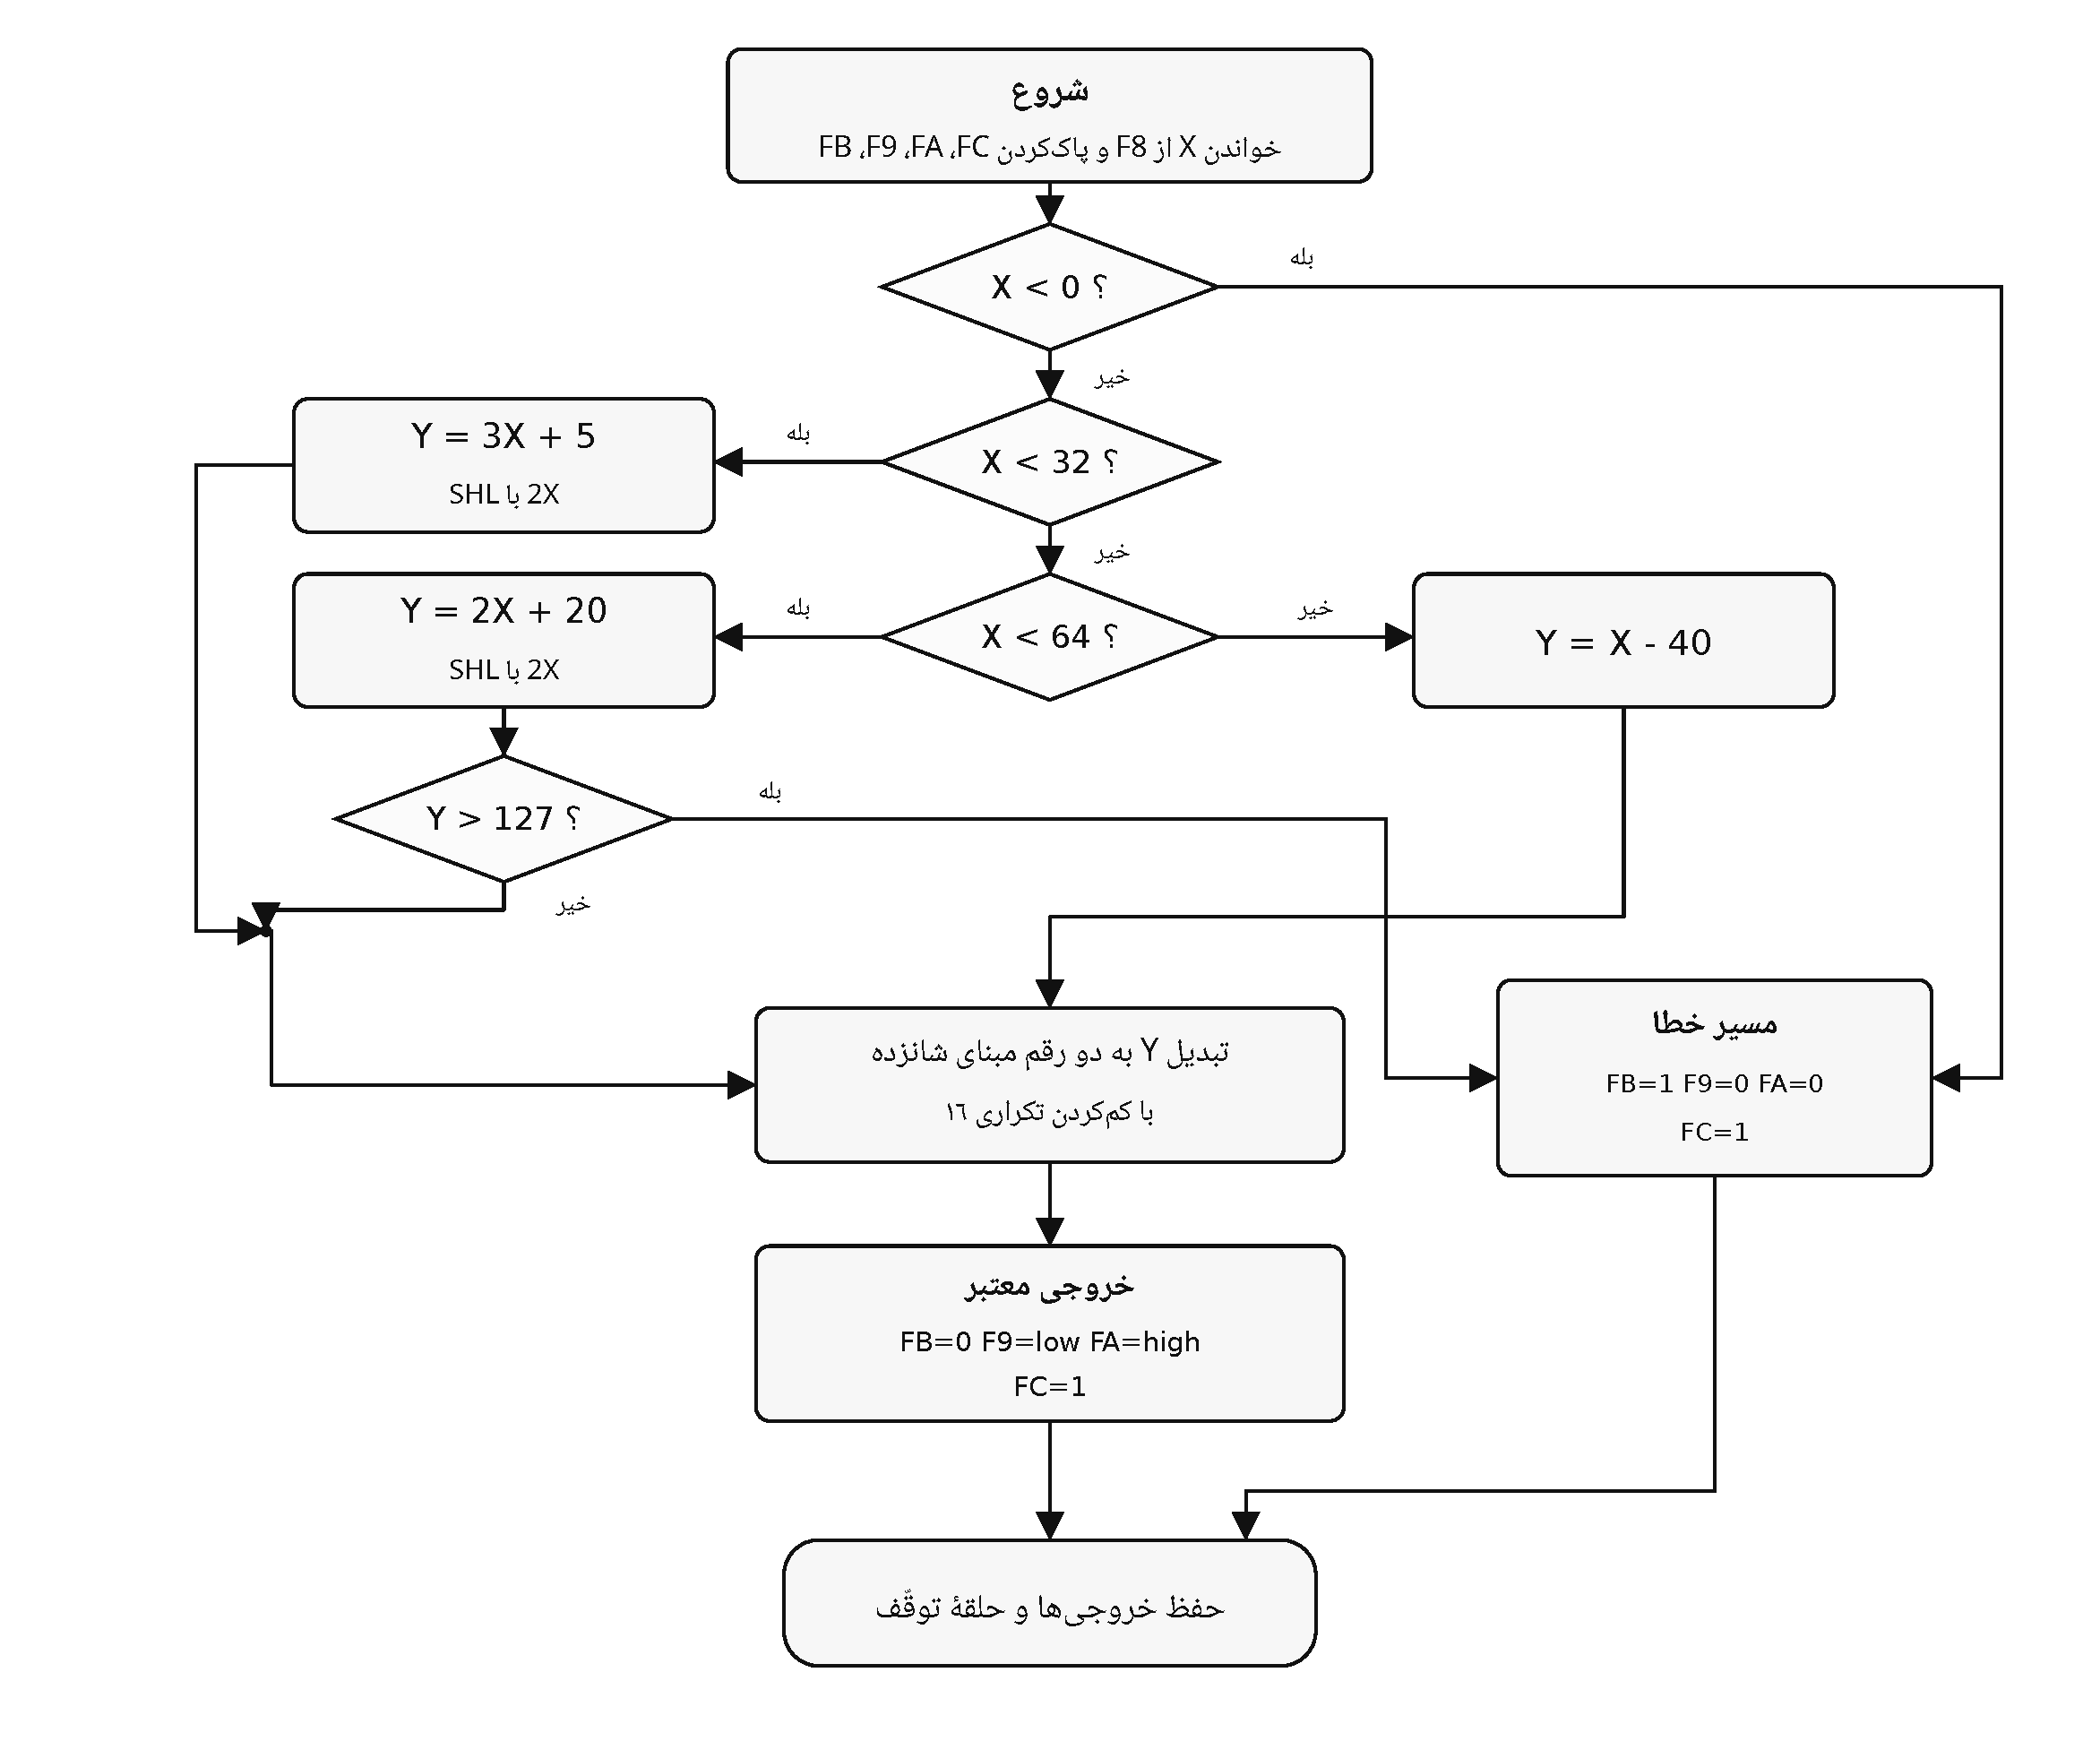
\includegraphics[width=0.96\textwidth,keepaspectratio]{images/program_flowchart.pdf}
  \caption{نمودار روند برنامۀ محاسبۀ تابع چندبخشی}
  \label{fig:program-flow}
\end{figure}

\subsection{جدول کامل کد ماشین}

جدول \ref{tab:machine-code} تمام دستورهای اجرایی برنامۀ \filename{program.hex} از نشانی \code{00} تا \code{AA} را نشان می‌دهد. خانه‌های \code{AB} تا \code{F7} برای تکمیل حافظۀ عادی با \code{00} پر شده‌اند و به دلیل حلقۀ توقّف در \code{A8--AA} هرگز اجرا نمی‌شوند.

\begingroup
\scriptsize
\setlength{\tabcolsep}{3pt}
\begin{longtable}{>{\centering\arraybackslash}p{1.0cm}
                  >{\centering\arraybackslash}p{1.8cm}
                  >{\centering\arraybackslash}p{2.5cm}
                  p{8.3cm}}
\caption{محتوای کامل بخش اجرایی حافظۀ برنامه}
\label{tab:machine-code}\\
\toprule
\textbf{نشانی} & \textbf{کد ماشین} & \textbf{دستور} & \textbf{توضیح} \\
\midrule
\endfirsthead
\toprule
\textbf{نشانی} & \textbf{کد ماشین} & \textbf{دستور} & \textbf{توضیح} \\
\midrule
\endhead
\lr{\texttt{00}} & \lr{\texttt{00 00}} & \lr{\texttt{PUSHC 00}} & صفرکردن مقدار اوّلیۀ خطا \\
\lr{\texttt{02}} & \lr{\texttt{02 FB}} & \lr{\texttt{POP FB}} & نوشتن صفر در درگاه خطا \\
\lr{\texttt{04}} & \lr{\texttt{00 00}} & \lr{\texttt{PUSHC 00}} & آماده‌سازی صفر برای رقم کم‌ارزش \\
\lr{\texttt{06}} & \lr{\texttt{02 F9}} & \lr{\texttt{POP F9}} & پاک‌کردن رقم کم‌ارزش نمایشگر \\
\lr{\texttt{08}} & \lr{\texttt{00 00}} & \lr{\texttt{PUSHC 00}} & آماده‌سازی صفر برای رقم پرارزش \\
\lr{\texttt{0A}} & \lr{\texttt{02 FA}} & \lr{\texttt{POP FA}} & پاک‌کردن رقم پرارزش نمایشگر \\
\lr{\texttt{0C}} & \lr{\texttt{00 00}} & \lr{\texttt{PUSHC 00}} & آماده‌سازی صفر برای پایان \\
\lr{\texttt{0E}} & \lr{\texttt{02 FC}} & \lr{\texttt{POP FC}} & صفرکردن چراغ پایان \\
\lr{\texttt{10}} & \lr{\texttt{01 F8}} & \lr{\texttt{PUSH F8}} & خواندن ورودی X \\
\lr{\texttt{12}} & \lr{\texttt{02 E0}} & \lr{\texttt{POP E0}} & ذخیرۀ X در خانۀ موقّت E0 \\
\lr{\texttt{14}} & \lr{\texttt{01 E0}} & \lr{\texttt{PUSH E0}} & قرار دادن X برای مقایسه با صفر \\
\lr{\texttt{16}} & \lr{\texttt{00 00}} & \lr{\texttt{PUSHC 00}} & قرار دادن صفر روی پشته \\
\lr{\texttt{18}} & \lr{\texttt{0A}} & \lr{\texttt{CMP}} & محاسبۀ موقّت X-0 و به‌روزرسانی پرچم‌ها \\
\lr{\texttt{19}} & \lr{\texttt{02 E3}} & \lr{\texttt{POP E3}} & حذف عملوند اوّل مقایسه \\
\lr{\texttt{1B}} & \lr{\texttt{02 E3}} & \lr{\texttt{POP E3}} & حذف عملوند دوّم مقایسه \\
\lr{\texttt{1D}} & \lr{\texttt{00 95}} & \lr{\texttt{PUSHC 95}} & قرار دادن نشانی مسیر خطا \\
\lr{\texttt{1F}} & \lr{\texttt{05}} & \lr{\texttt{JS}} & پرش به خطا در صورت منفی‌بودن X \\
\lr{\texttt{20}} & \lr{\texttt{01 E0}} & \lr{\texttt{PUSH E0}} & قرار دادن X برای مقایسه با 32 \\
\lr{\texttt{22}} & \lr{\texttt{00 20}} & \lr{\texttt{PUSHC 20}} & قرار دادن 32 روی پشته \\
\lr{\texttt{24}} & \lr{\texttt{0A}} & \lr{\texttt{CMP}} & مقایسۀ X با 32 \\
\lr{\texttt{25}} & \lr{\texttt{02 E3}} & \lr{\texttt{POP E3}} & پاک‌سازی عملوند مقایسه \\
\lr{\texttt{27}} & \lr{\texttt{02 E3}} & \lr{\texttt{POP E3}} & پاک‌سازی عملوند مقایسه \\
\lr{\texttt{29}} & \lr{\texttt{00 3B}} & \lr{\texttt{PUSHC 3B}} & قرار دادن نشانی بازۀ اوّل \\
\lr{\texttt{2B}} & \lr{\texttt{05}} & \lr{\texttt{JS}} & اگر X<32 باشد، پرش به بازۀ اوّل \\
\lr{\texttt{2C}} & \lr{\texttt{01 E0}} & \lr{\texttt{PUSH E0}} & قرار دادن X برای مقایسه با 64 \\
\lr{\texttt{2E}} & \lr{\texttt{00 40}} & \lr{\texttt{PUSHC 40}} & قرار دادن 64 روی پشته \\
\lr{\texttt{30}} & \lr{\texttt{0A}} & \lr{\texttt{CMP}} & مقایسۀ X با 64 \\
\lr{\texttt{31}} & \lr{\texttt{02 E3}} & \lr{\texttt{POP E3}} & پاک‌سازی عملوند مقایسه \\
\lr{\texttt{33}} & \lr{\texttt{02 E3}} & \lr{\texttt{POP E3}} & پاک‌سازی عملوند مقایسه \\
\lr{\texttt{35}} & \lr{\texttt{00 49}} & \lr{\texttt{PUSHC 49}} & قرار دادن نشانی بازۀ دوّم \\
\lr{\texttt{37}} & \lr{\texttt{05}} & \lr{\texttt{JS}} & اگر X<64 باشد، پرش به بازۀ دوّم \\
\lr{\texttt{38}} & \lr{\texttt{00 57}} & \lr{\texttt{PUSHC 57}} & قرار دادن نشانی بازۀ سوّم \\
\lr{\texttt{3A}} & \lr{\texttt{03}} & \lr{\texttt{JUMP}} & پرش بدون شرط به بازۀ سوّم \\
\lr{\texttt{3B}} & \lr{\texttt{01 E0}} & \lr{\texttt{PUSH E0}} & خواندن X برای بازۀ اوّل \\
\lr{\texttt{3D}} & \lr{\texttt{09}} & \lr{\texttt{SHL}} & محاسبۀ 2X با انتقال یک‌بیتی به چپ \\
\lr{\texttt{3E}} & \lr{\texttt{01 E0}} & \lr{\texttt{PUSH E0}} & قرار دادن X روی پشته \\
\lr{\texttt{40}} & \lr{\texttt{06}} & \lr{\texttt{ADD}} & محاسبۀ 3X = 2X + X \\
\lr{\texttt{41}} & \lr{\texttt{00 05}} & \lr{\texttt{PUSHC 05}} & قرار دادن ثابت 5 \\
\lr{\texttt{43}} & \lr{\texttt{06}} & \lr{\texttt{ADD}} & محاسبۀ Y=3X+5 \\
\lr{\texttt{44}} & \lr{\texttt{02 E1}} & \lr{\texttt{POP E1}} & ذخیرۀ Y در E1 \\
\lr{\texttt{46}} & \lr{\texttt{00 61}} & \lr{\texttt{PUSHC 61}} & قرار دادن نشانی بخش تبدیل خروجی \\
\lr{\texttt{48}} & \lr{\texttt{03}} & \lr{\texttt{JUMP}} & پرش به بخش تبدیل مبنای شانزده \\
\lr{\texttt{49}} & \lr{\texttt{01 E0}} & \lr{\texttt{PUSH E0}} & خواندن X برای بازۀ دوّم \\
\lr{\texttt{4B}} & \lr{\texttt{09}} & \lr{\texttt{SHL}} & محاسبۀ 2X با SHL \\
\lr{\texttt{4C}} & \lr{\texttt{00 14}} & \lr{\texttt{PUSHC 14}} & قرار دادن ثابت 20 ده‌دهی \\
\lr{\texttt{4E}} & \lr{\texttt{06}} & \lr{\texttt{ADD}} & محاسبۀ Y=2X+20 و تعیین پرچم علامت \\
\lr{\texttt{4F}} & \lr{\texttt{02 E1}} & \lr{\texttt{POP E1}} & ذخیرۀ Y بدون تغییر پرچم‌ها \\
\lr{\texttt{51}} & \lr{\texttt{00 95}} & \lr{\texttt{PUSHC 95}} & قرار دادن نشانی خطا \\
\lr{\texttt{53}} & \lr{\texttt{05}} & \lr{\texttt{JS}} & تشخیص Y>127 از بیت علامت و پرش به خطا \\
\lr{\texttt{54}} & \lr{\texttt{00 61}} & \lr{\texttt{PUSHC 61}} & قرار دادن نشانی بخش تبدیل خروجی \\
\lr{\texttt{56}} & \lr{\texttt{03}} & \lr{\texttt{JUMP}} & پرش به بخش تبدیل مبنای شانزده \\
\lr{\texttt{57}} & \lr{\texttt{01 E0}} & \lr{\texttt{PUSH E0}} & خواندن X برای بازۀ سوّم \\
\lr{\texttt{59}} & \lr{\texttt{00 28}} & \lr{\texttt{PUSHC 28}} & قرار دادن ثابت 40 ده‌دهی \\
\lr{\texttt{5B}} & \lr{\texttt{07}} & \lr{\texttt{SUB}} & محاسبۀ Y=X-40 بر پایۀ B-A \\
\lr{\texttt{5C}} & \lr{\texttt{02 E1}} & \lr{\texttt{POP E1}} & ذخیرۀ Y در E1 \\
\lr{\texttt{5E}} & \lr{\texttt{00 61}} & \lr{\texttt{PUSHC 61}} & قرار دادن نشانی بخش تبدیل خروجی \\
\lr{\texttt{60}} & \lr{\texttt{03}} & \lr{\texttt{JUMP}} & پرش به بخش تبدیل مبنای شانزده \\
\lr{\texttt{61}} & \lr{\texttt{00 00}} & \lr{\texttt{PUSHC 00}} & مقداردهی اوّلیۀ رقم پرارزش \\
\lr{\texttt{63}} & \lr{\texttt{02 E2}} & \lr{\texttt{POP E2}} & E2=0 \\
\lr{\texttt{65}} & \lr{\texttt{01 E1}} & \lr{\texttt{PUSH E1}} & قرار دادن باقیماندۀ جاری روی پشته \\
\lr{\texttt{67}} & \lr{\texttt{00 10}} & \lr{\texttt{PUSHC 10}} & قرار دادن 16 ده‌دهی \\
\lr{\texttt{69}} & \lr{\texttt{0A}} & \lr{\texttt{CMP}} & مقایسۀ باقیمانده با 16 \\
\lr{\texttt{6A}} & \lr{\texttt{02 E3}} & \lr{\texttt{POP E3}} & پاک‌سازی عملوند مقایسه \\
\lr{\texttt{6C}} & \lr{\texttt{02 E3}} & \lr{\texttt{POP E3}} & پاک‌سازی عملوند مقایسه \\
\lr{\texttt{6E}} & \lr{\texttt{00 82}} & \lr{\texttt{PUSHC 82}} & قرار دادن نشانی پایان تبدیل \\
\lr{\texttt{70}} & \lr{\texttt{05}} & \lr{\texttt{JS}} & اگر باقیمانده<16 باشد، پایان حلقه \\
\lr{\texttt{71}} & \lr{\texttt{01 E1}} & \lr{\texttt{PUSH E1}} & خواندن باقیماندۀ جاری \\
\lr{\texttt{73}} & \lr{\texttt{00 10}} & \lr{\texttt{PUSHC 10}} & قرار دادن 16 \\
\lr{\texttt{75}} & \lr{\texttt{07}} & \lr{\texttt{SUB}} & کم‌کردن 16 از باقیمانده \\
\lr{\texttt{76}} & \lr{\texttt{02 E1}} & \lr{\texttt{POP E1}} & ذخیرۀ باقیماندۀ جدید \\
\lr{\texttt{78}} & \lr{\texttt{01 E2}} & \lr{\texttt{PUSH E2}} & خواندن رقم پرارزش جاری \\
\lr{\texttt{7A}} & \lr{\texttt{00 01}} & \lr{\texttt{PUSHC 01}} & قرار دادن ثابت یک \\
\lr{\texttt{7C}} & \lr{\texttt{06}} & \lr{\texttt{ADD}} & افزایش رقم پرارزش \\
\lr{\texttt{7D}} & \lr{\texttt{02 E2}} & \lr{\texttt{POP E2}} & ذخیرۀ رقم پرارزش جدید \\
\lr{\texttt{7F}} & \lr{\texttt{00 65}} & \lr{\texttt{PUSHC 65}} & قرار دادن نشانی ابتدای حلقه \\
\lr{\texttt{81}} & \lr{\texttt{03}} & \lr{\texttt{JUMP}} & تکرار حلقۀ تبدیل \\
\lr{\texttt{82}} & \lr{\texttt{00 00}} & \lr{\texttt{PUSHC 00}} & آماده‌سازی صفر برای خطا \\
\lr{\texttt{84}} & \lr{\texttt{02 FB}} & \lr{\texttt{POP FB}} & خاموش‌کردن چراغ خطا \\
\lr{\texttt{86}} & \lr{\texttt{01 E1}} & \lr{\texttt{PUSH E1}} & خواندن رقم کم‌ارزش \\
\lr{\texttt{88}} & \lr{\texttt{02 F9}} & \lr{\texttt{POP F9}} & نوشتن رقم کم‌ارزش در F9 \\
\lr{\texttt{8A}} & \lr{\texttt{01 E2}} & \lr{\texttt{PUSH E2}} & خواندن رقم پرارزش \\
\lr{\texttt{8C}} & \lr{\texttt{02 FA}} & \lr{\texttt{POP FA}} & نوشتن رقم پرارزش در FA \\
\lr{\texttt{8E}} & \lr{\texttt{00 01}} & \lr{\texttt{PUSHC 01}} & آماده‌سازی علامت پایان \\
\lr{\texttt{90}} & \lr{\texttt{02 FC}} & \lr{\texttt{POP FC}} & روشن‌کردن چراغ پایان \\
\lr{\texttt{92}} & \lr{\texttt{00 A8}} & \lr{\texttt{PUSHC A8}} & قرار دادن نشانی توقّف \\
\lr{\texttt{94}} & \lr{\texttt{03}} & \lr{\texttt{JUMP}} & ورود به حلقۀ توقّف \\
\lr{\texttt{95}} & \lr{\texttt{00 01}} & \lr{\texttt{PUSHC 01}} & آماده‌سازی مقدار خطا \\
\lr{\texttt{97}} & \lr{\texttt{02 FB}} & \lr{\texttt{POP FB}} & روشن‌کردن چراغ خطا \\
\lr{\texttt{99}} & \lr{\texttt{00 00}} & \lr{\texttt{PUSHC 00}} & آماده‌سازی صفر برای نمایشگر \\
\lr{\texttt{9B}} & \lr{\texttt{02 F9}} & \lr{\texttt{POP F9}} & پاک‌کردن رقم کم‌ارزش \\
\lr{\texttt{9D}} & \lr{\texttt{00 00}} & \lr{\texttt{PUSHC 00}} & آماده‌سازی صفر برای نمایشگر \\
\lr{\texttt{9F}} & \lr{\texttt{02 FA}} & \lr{\texttt{POP FA}} & پاک‌کردن رقم پرارزش \\
\lr{\texttt{A1}} & \lr{\texttt{00 01}} & \lr{\texttt{PUSHC 01}} & آماده‌سازی علامت پایان \\
\lr{\texttt{A3}} & \lr{\texttt{02 FC}} & \lr{\texttt{POP FC}} & روشن‌کردن چراغ پایان \\
\lr{\texttt{A5}} & \lr{\texttt{00 A8}} & \lr{\texttt{PUSHC A8}} & قرار دادن نشانی توقّف \\
\lr{\texttt{A7}} & \lr{\texttt{03}} & \lr{\texttt{JUMP}} & ورود به حلقۀ توقّف \\
\lr{\texttt{A8}} & \lr{\texttt{00 A8}} & \lr{\texttt{PUSHC A8}} & قرار دادن نشانی خود حلقه \\
\lr{\texttt{AA}} & \lr{\texttt{03}} & \lr{\texttt{JUMP}} & پرش به A8 و نگه‌داشتن خروجی‌ها \\
\bottomrule
\end{longtable}
\endgroup

\section{سنتز و مشاهدۀ ساختار در \lr{Quartus}}

\subsection{روند انجام کار در \lr{Quartus}}

فایل‌های \lr{\texttt{stack\_cpu.v}}، \lr{\texttt{memory\_io.v}}، \lr{\texttt{processor\_system.v}}، \lr{\texttt{seven\_segment\_decoder.v}} و \lr{\texttt{stack\_processor\_top.v}} به پروژه افزوده شدند و \lr{\texttt{stack\_processor\_top.v}} به‌عنوان موجودیت سطح بالا انتخاب شد. برای کامپایل کامل پروژه از مسیر زیر استفاده شد:

\begin{latin}
\begin{center}
\texttt{Processing > Start Compilation}
\end{center}
\end{latin}

پس از پایان کامپایل، برای مشاهدۀ نمای سطح انتقال ثبات\enfoot{Register-Transfer Level (RTL)} مسیر زیر در \lr{Quartus} استفاده شد:

\begin{latin}
\begin{center}
\texttt{Tools > Netlist Viewers > RTL Viewer}
\end{center}
\end{latin}

نمای سطح انتقال ثبات حاصل از سنتز\enfoot{Synthesis}، ارتباط واقعی پیمانه‌ها و منطق استخراج‌شده از توصیف \lr{Verilog} را نمایش می‌دهد.

\subsection{نمای سطح بالای سامانه}

\begin{figure}[H]
  \centering
  \reportimage{images/image01.png}
  \caption{نمای \lr{RTL} سطح بالای \lr{\texttt{stack\_processor\_top.v}}}
  \label{fig:rtl-top}
\end{figure}

در شکل \ref{fig:rtl-top} پیمانۀ \code{processor_system} در سمت چپ و دو رمزگشای نمایشگر در سمت راست دیده می‌شوند. دو رقم داخلی \code{hex_high} و \code{hex_low} از سامانهٔ پردازنده خارج شده و به رمزگشاها می‌روند؛ درحالی‌که \code{error_led} و \code{done_led} مستقیماً به خروجی سطح بالا متصل هستند.

\subsection{نمای تفصیلی پردازنده}

\begin{figure}[H]
  \centering
  \reportimage{images/image02.png}
  \caption{نمای \lr{RTL} تفصیلی پردازنده پس از سنتز}
  \label{fig:rtl-cpu}
\end{figure}

شکل \ref{fig:rtl-cpu} نمای تفصیلی منطق سنتزشده را نشان می‌دهد. شلوغی این نما طبیعی است؛ زیرا پشته، ماشین حالت، منطق نشانی‌دهی حافظه، جمع و تفریق، مسیرهای دستورهای جدید و ثبات‌های وضعیّت همگی به عناصر منطقی صریح تبدیل شده‌اند. این تصویر در کنار نمودار بلوکی شکل \ref{fig:block-diagram} هم ساختار مفهومی و هم ساختار واقعی حاصل از سنتز را پوشش می‌دهد.

\subsection{نتیجۀ کامپایل}

\begin{figure}[H]
  \centering
  \reportimage{images/image03.png}
  \caption{خروجی \lr{Quartus} و موفّقیت کامپایل کامل پروژه}
  \label{fig:quartus-compile}
\end{figure}

همان‌طور که در شکل \ref{fig:quartus-compile} دیده می‌شود، کامپایل کامل با صفر خطا پایان یافته است. هشدارهای زمان‌بندی موجود در تصویر به نبود فایل قیود زمانی و مشخّص‌نشدن قید واقعی ساعت مربوط‌اند و مانع انجام تحلیل و سنتز، جانمایی و مسیریابی و تولید خروجی کامپایل نشده‌اند. بنابراین از دید \lr{Quartus} طراحی قابل سنتز است.

\section{طراحی و روش کار فایل‌های آزمون}

در این پروژه دو فایل آزمون\enfoot{Testbench} مستقل وجود دارد. کد این فایل‌ها در گزارش درج نشده است، امّا هر دو همراه پروژه تحویل داده می‌شوند و نحوۀ آزمون آن‌ها در ادامه به‌صورت کامل توضیح داده شده است.

\subsection{آزمون مستقل دستورهای جدید در \lr{\texttt{stack\_cpu\_tb.v}}}

این فایل مستقیماً \lr{\texttt{stack\_cpu.v}} را نمونه‌سازی می‌کند و یک مدل سادۀ حافظه در کنار آن قرار می‌دهد. برای هر آزمون، یک برنامۀ بسیار کوتاه در حافظۀ مدل نوشته می‌شود، پردازنده بازنشانی می‌گردد و پس از پایان دستور مورد نظر، محتوای پشته و در صورت نیاز پرچم‌ها بررسی می‌شوند.

\subsubsection{آزمون \lr{SWAP}}

دو مقدار متفاوت \code{12} و \code{A5} به‌ترتیب روی پشته قرار می‌گیرند. پیش از \code{SWAP}، مقدار \code{A5} به‌عنوان \(A\) در بالای پشته و مقدار \code{12} به‌عنوان \(B\) در جایگاه دوّم قرار دارد. پس از اجرای دستور انتظار می‌رود عنصر بالا \code{12} و عنصر دوّم \code{A5} باشد و عمق پشته همچنان دو باقی بماند. این آزمون الزام مستقل دستور \code{SWAP} را پوشش می‌دهد؛ هرچند استفاده از این دستور در برنامۀ نهایی برای تابع ضروری نیست.

\subsubsection{آزمون‌های \lr{SHL}}

چهار مقدار الزام‌شده در صورت آزمایش بررسی شده‌اند:
\[
0\rightarrow 0,\qquad
1\rightarrow 2,\qquad
63\rightarrow126,\qquad
127\rightarrow254.
\]
در هر چهار حالت، یک مقدار روی پشته قرار گرفته، \code{SHL} اجرا و مقدار جدید بالای پشته با نتیجۀ مورد انتظار مقایسه می‌شود. عمق پشته باید یک باقی بماند.

\subsubsection{آزمون‌های \lr{CMP}}

سه حالت مورد نیاز با تعریف \(T=B-A\) بررسی شده‌اند:
\begin{itemize}[itemsep=0.25em]
  \item \(B<A\): با \(B=5\) و \(A=9\)، داریم \(T=-4\)، پس \code{Z=0} و \code{S=1}.
  \item \(B=A\): با \(B=7\) و \(A=7\)، داریم \(T=0\)، پس \code{Z=1} و \code{S=0}.
  \item \(B>A\): با \(B=9\) و \(A=5\)، داریم \(T=4\)، پس \code{Z=0} و \code{S=0}.
\end{itemize}
علاوه بر پرچم‌ها، آزمون بررسی می‌کند که هر دو مقدار روی پشته بدون تغییر باقی مانده باشند.

\begin{figure}[H]
  \centering
  \reportimage{images/image04.png}
  \caption{خروجی آزمون مستقل \lr{SWAP}، \lr{SHL} و \lr{CMP}}
  \label{fig:cpu-tests}
\end{figure}

شکل \ref{fig:cpu-tests} نشان می‌دهد هر هشت آزمون مستقل موفّق بوده‌اند:
\begin{latin}
\begin{center}
\texttt{Passed: 8 \qquad Failed: 0}
\end{center}
\end{latin}

\subsection{آزمون برنامۀ کامل در \lr{\texttt{stack\_processor\_top\_tb.v}}}

فایل آزمون دوّم کل سامانه، شامل پردازنده، حافظه، برنامۀ زبان ماشین، منطق ورودی و خروجی و دو رمزگشای نمایشگر را بررسی می‌کند. برای هر ورودی، ابتدا مقدار مرجع تابع در خود فایل آزمون محاسبه می‌شود. سپس \(X\) روی ورودی قرار گرفته، بازنشانی اعمال می‌شود و فایل آزمون تا یک‌شدن \code{done_led} منتظر می‌ماند. پس از آن موارد زیر با مقدار مورد انتظار مقایسه می‌شوند:
\begin{itemize}[itemsep=0.25em]
  \item \code{error_led}؛
  \item رقم پرارزش و کم‌ارزش مبنای شانزده؛
  \item الگوی هفت‌بیتی هر دو نمایشگر هفت‌قسمتی.
\end{itemize}

استفاده از عملگر ضرب در محاسبۀ \emph{مقدار مرجع} فایل آزمون، بخشی از سخت‌افزار قابل سنتز نیست و فقط برای مقایسۀ خودکار نتیجۀ پردازنده استفاده می‌شود. در برنامۀ زبان ماشین و کدهای اصلی قابل سنتز، محاسبۀ \(2X\) با \code{SHL} و \(3X\) با \(X+2X\) انجام شده است.

خروجی نمایشگرها فعّال‌پایین است. الگوهای لازم برای ارقامی که در آزمون‌های الزامی ظاهر می‌شوند در جدول \ref{tab:segment-patterns} آمده‌اند.

\begin{table}[H]
\centering
\small
\begin{tabular}{c c c}
\toprule
\textbf{رقم} & \textbf{الگوی هفت‌بیتی} & \textbf{نمایش شانزدهی الگو} \\
\midrule
0 & \lr{\texttt{1000000}} & \lr{\texttt{0x40}} \\
1 & \lr{\texttt{1111001}} & \lr{\texttt{0x79}} \\
2 & \lr{\texttt{0100100}} & \lr{\texttt{0x24}} \\
4 & \lr{\texttt{0011001}} & \lr{\texttt{0x19}} \\
5 & \lr{\texttt{0010010}} & \lr{\texttt{0x12}} \\
6 & \lr{\texttt{0000010}} & \lr{\texttt{0x02}} \\
7 & \lr{\texttt{1111000}} & \lr{\texttt{0x78}} \\
8 & \lr{\texttt{0000000}} & \lr{\texttt{0x00}} \\
E & \lr{\texttt{0000110}} & \lr{\texttt{0x06}} \\
\bottomrule
\end{tabular}
\caption{الگوهای نمایشگر هفت‌قسمتی مورد استفاده در آزمون‌های الزامی}
\label{tab:segment-patterns}
\end{table}

\section{توضیح کامل آزمون‌های الزامی برنامۀ نهایی}

\subsection{ورودی \(X=0\)}

این مقدار کوچک‌ترین ورودی معتبر و در ابتدای بازۀ اوّل است. با مقایسۀ \(0\) و \(32\)، پرچم علامت برای \(0-32\) یک می‌شود و برنامه به مسیر اوّل می‌رود:
\[
Y=3(0)+5=5=05_{16}.
\]
پس رقم پرارزش \(0\) و رقم کم‌ارزش \(5\) است. خروجی واقعی دو رمزگشا به‌ترتیب
\code{seven_segment_high=1000000 (0x40)}
و
\code{seven_segment_low=0010010 (0x12)}
خواهد بود. \code{error_led=0} و پس از تکمیل نوشتن خروجی‌ها \code{done_led=1} می‌شود.

\subsection{ورودی \(X=31\)}

این مقدار آخرین عضو بازۀ اوّل است:
\[
Y=3(31)+5=98=62_{16}.
\]
بنابراین رقم پرارزش \(6\) و رقم کم‌ارزش \(2\) است و الگوهای هفت‌بیتی به‌ترتیب
\code{0000010 (0x02)}
و
\code{0100100 (0x24)}
هستند.
خروجی معتبر است، پس خطا صفر و پایان در انتهای محاسبه یک می‌شود.

\subsection{ورودی \(X=32\)}

این مقدار نخستین عضو بازۀ دوّم است. مقایسۀ اوّل نشان می‌دهد \(X<32\) برقرار نیست و مقایسۀ دوّم، \(X<64\) را تأیید می‌کند:
\[
Y=2(32)+20=84=54_{16}.
\]
رقم پرارزش \(5\) با الگوی \code{0010010} یا \code{0x12} و رقم کم‌ارزش \(4\) با الگوی \code{0011001} یا \code{0x19} نمایش داده می‌شود. خطا صفر است.

\subsection{ورودی \(X=53\)}

این مقدار بزرگ‌ترین خروجی معتبر بازۀ دوّم را ایجاد می‌کند:
\[
Y=2(53)+20=126=7E_{16}.
\]
بیت علامت نتیجۀ هشت‌بیتی صفر است؛ بنابراین مسیر خطا انتخاب نمی‌شود. رقم پرارزش \(7\) و رقم کم‌ارزش \(E\) هستند. الگوی رقم پرارزش
\code{1111000 (0x78)}
و الگوی رقم کم‌ارزش
\code{0000110 (0x06)}
است.
\code{error_led=0} و \code{done_led=1} در پایان برقرار می‌شوند.

\subsection{ورودی \(X=54\)}

این ورودی نخستین مقدار بازۀ دوّم است که خروجی ریاضی آن از ۱۲۷ بزرگ‌تر می‌شود:
\[
Y=2(54)+20=128.
\]
عدد ۱۲۸ در نتیجۀ هشت‌بیتی دارای بیت شمارۀ هفت برابر یک است؛ بنابراین بعد از \code{ADD}، پرچم \code{S} یک شده و \code{JS} مسیر خطا را انتخاب می‌کند. در مسیر خطا مقدار ریاضی ۱۲۸ روی نمایشگر قرار نمی‌گیرد؛ بلکه هر دو رقم صفر می‌شوند. بنابراین
\code{HEX=00}
و الگوی هر دو نمایشگر
\code{1000000 (0x40)}
است.
هم‌زمان \code{error_led=1} و در پایان \code{done_led=1} می‌شود.

\subsection{ورودی \(X=63\)}

این مقدار آخرین عضو بازۀ دوّم است:
\[
Y=2(63)+20=146>127.
\]
در نتیجه همانند آزمون قبل، مسیر خطا اجرا می‌شود. خروجی دو نمایشگر \code{00}، هر دو الگوی هفت‌بیتی \code{0x40}، خطا برابر یک و پایان برابر یک خواهد بود.

\subsection{ورودی \(X=64\)}

این مقدار نخستین عضو بازۀ سوّم است:
\[
Y=64-40=24=18_{16}.
\]
رقم پرارزش \(1\) با الگوی
\[
1111001=0x79
\]
و رقم کم‌ارزش \(8\) با الگوی
\[
0000000=0x00
\]
نمایش داده می‌شود. خروجی معتبر است؛ بنابراین خطا صفر و پایان یک است.

\subsection{ورودی \(X=127\)}

این مقدار بزرگ‌ترین ورودی مثبت هشت‌بیتی علامت‌دار است و در بازۀ سوّم قرار دارد:
\[
Y=127-40=87=57_{16}.
\]
رقم پرارزش \(5\) با الگوی \code{0x12} و رقم کم‌ارزش \(7\) با الگوی \code{0x78} نمایش داده می‌شود. \code{error_led=0} و \code{done_led=1} است.

\subsection{ورودی \(X=128\)}

الگوی هشت‌بیتی \code{10000000} در نمایش متمّم دو برابر \(-128\) است. از آنجا که بیت شمارۀ هفت ورودی یک است، برنامه قبل از ورود به هر بازۀ تابع، ورودی را نامعتبر تشخیص داده و به مسیر خطا می‌رود. خروجی دو نمایشگر \code{00} است و الگوی هر دو نمایشگر \code{0x40} خواهد بود. همچنین \code{error_led=1} و \code{done_led=1} می‌شوند.

\subsection{ورودی \(X=255\)}

الگوی \code{11111111} در نمایش متمّم دو برابر \(-1\) است؛ بنابراین همان بررسی اوّلیۀ علامت، ورودی را نامعتبر تشخیص می‌دهد. هیچ‌یک از سه رابطۀ تابع اجرا نمی‌شوند. نمایشگرها \code{00}، خطا یک و پایان یک خواهند بود.

\begin{table}[H]
\centering
\scriptsize
\begin{tabularx}{\textwidth}{>{\centering\arraybackslash}p{0.9cm}
                            >{\centering\arraybackslash}p{1.6cm}
                            >{\centering\arraybackslash}p{1.2cm}
                            >{\centering\arraybackslash}p{1.2cm}
                            >{\centering\arraybackslash}p{2.0cm}
                            >{\centering\arraybackslash}p{2.0cm}
                            >{\centering\arraybackslash}p{1.0cm}
                            >{\centering\arraybackslash}p{1.0cm}}
\toprule
\(X\) & نتیجۀ ریاضی & \(\mathrm{HEX}\) & خطا &
الگوی پرارزش & الگوی کم‌ارزش & خطا & پایان \\
\midrule
0   & 5   & \lr{\texttt{05}} & خیر & \lr{\texttt{0x40}} & \lr{\texttt{0x12}} & 0 & 1 \\
31  & 98  & \lr{\texttt{62}} & خیر & \lr{\texttt{0x02}} & \lr{\texttt{0x24}} & 0 & 1 \\
32  & 84  & \lr{\texttt{54}} & خیر & \lr{\texttt{0x12}} & \lr{\texttt{0x19}} & 0 & 1 \\
53  & 126 & \lr{\texttt{7E}} & خیر & \lr{\texttt{0x78}} & \lr{\texttt{0x06}} & 0 & 1 \\
54  & 128 & \lr{\texttt{00}} & بله & \lr{\texttt{0x40}} & \lr{\texttt{0x40}} & 1 & 1 \\
63  & 146 & \lr{\texttt{00}} & بله & \lr{\texttt{0x40}} & \lr{\texttt{0x40}} & 1 & 1 \\
64  & 24  & \lr{\texttt{18}} & خیر & \lr{\texttt{0x79}} & \lr{\texttt{0x00}} & 0 & 1 \\
127 & 87  & \lr{\texttt{57}} & خیر & \lr{\texttt{0x12}} & \lr{\texttt{0x78}} & 0 & 1 \\
128 & نامعتبر & \lr{\texttt{00}} & بله & \lr{\texttt{0x40}} & \lr{\texttt{0x40}} & 1 & 1 \\
255 & نامعتبر & \lr{\texttt{00}} & بله & \lr{\texttt{0x40}} & \lr{\texttt{0x40}} & 1 & 1 \\
\bottomrule
\end{tabularx}
\caption{خلاصۀ خروجی ده آزمون الزامی}
\label{tab:mandatory-tests}
\end{table}

\begin{figure}[H]
  \centering
  \reportimage{images/image05.png}
  \caption{خروجی فایل آزمون برنامۀ کامل؛ ده آزمون الزامی و پیمایش جامع ۲۵۶ ورودی}
  \label{fig:system-tests}
\end{figure}

در شکل \ref{fig:system-tests} تمام ده ورودی الزام‌شده با نتیجۀ مورد انتظار موفّق شده‌اند. پس از آن نیز تمامی ۲۵۶ الگوی ممکن ورودی هشت‌بیتی از صفر تا ۲۵۵ بررسی شده‌اند. در مجموع ۲۶۶ اجرای مستقل انجام شده و نتیجه برابر است با
\begin{latin}
\begin{center}
\texttt{Passed: 266 \qquad Failed: 0}
\end{center}
\end{latin}
این آزمون جامع نشان می‌دهد صحّت سامانه فقط به چند ورودی مرزی محدود نیست.

\section{شکل موج‌های منتخب و تحلیل آن‌ها}

از آنجا که ده آزمون الزامی و سپس ۲۵۶ آزمون جامع اجرا می‌شوند، قرار دادن شکل موج مستقل برای تمام اجراها باعث شلوغی بسیار زیاد گزارش می‌شود. بنابراین در این بخش فقط چند شکل موج\enfoot{Waveform} منتخب از مسیرهای مهم آورده شده‌اند. صحّت تمام ده آزمون در بخش قبل و در خروجی متنی شکل \ref{fig:system-tests} ثبت شده است.

در شکل موج‌ها، سیگنال‌های \code{seven_segment_high} و \code{seven_segment_low} خود \emph{عدد} نیستند؛ بلکه الگوی هفت‌بیتی فعّال‌پایین برای روشن و خاموش کردن قسمت‌های نمایشگر هستند. به همین دلیل برای نمونه نمایش رقم \(6\) به‌صورت \code{0x02} و نمایش رقم \(2\) به‌صورت \code{0x24} دیده می‌شود.

\subsection{شکل موج \(X=31\)}

\begin{figure}[H]
  \centering
  \reportimage{images/image06.png}
  \caption{شکل موج اجرای برنامه برای \(X=31\)}
  \label{fig:wave31}
\end{figure}

برای \(X=31\)، نتیجۀ تابع \(98=62_{16}\) است. در شکل \ref{fig:wave31} ابتدا رقم کم‌ارزش به \code{0x24}، یعنی الگوی رقم \(2\)، و سپس رقم پرارزش به \code{0x02}، یعنی الگوی رقم \(6\)، تغییر می‌کند. \code{error_led} صفر باقی می‌ماند و پس از تثبیت خروجی‌ها \code{done_led} یک می‌شود.

\subsection{شکل موج \(X=32\)}

\begin{figure}[H]
  \centering
  \reportimage{images/image07.png}
  \caption{شکل موج اجرای برنامه برای \(X=32\)}
  \label{fig:wave32}
\end{figure}

این ورودی نخستین عضو بازۀ دوّم است و خروجی \(84=54_{16}\) تولید می‌شود. الگوی رقم \(5\) برابر \code{0x12} و الگوی رقم \(4\) برابر \code{0x19} است. در شکل \ref{fig:wave32} هر دو مقدار پیش از فعّال‌شدن \code{done_led} روی خروجی قرار گرفته‌اند و خطا صفر است.

\subsection{شکل موج \(X=54\)}

\begin{figure}[H]
  \centering
  \reportimage{images/image08.png}
  \caption{شکل موج مسیر خطا برای \(X=54\)}
  \label{fig:wave54}
\end{figure}

برای \(X=54\)، خروجی ریاضی ۱۲۸ است و بنابراین سرریز\enfoot{Overflow} نسبت به بازۀ مجاز مثبت رخ می‌دهد. شکل \ref{fig:wave54} نشان می‌دهد \code{error_led} فعّال می‌شود و هر دو نمایشگر روی الگوی \code{0x40}، یعنی رقم صفر، باقی می‌مانند. در پایان \code{done_led} نیز یک می‌شود.

\subsection{شکل موج \(X=64\)}

\begin{figure}[H]
  \centering
  \reportimage{images/image09.png}
  \caption{شکل موج اجرای برنامه برای \(X=64\)}
  \label{fig:wave64}
\end{figure}

برای \(X=64\)، مسیر سوّم تابع اجرا می‌شود:
\[
Y=64-40=24=18_{16}.
\]
در نتیجه الگوی رقم پرارزش \(1\) برابر \code{0x79} و الگوی رقم کم‌ارزش \(8\) برابر \code{0x00} است. هر دو مقدار در شکل \ref{fig:wave64} دیده می‌شوند و خطا صفر باقی می‌ماند.

\subsection{شکل موج \(X=128\)}

\begin{figure}[H]
  \centering
  \reportimage{images/image10.png}
  \caption{شکل موج تشخیص ورودی منفی برای \(X=128\)}
  \label{fig:wave128}
\end{figure}

الگوی \(128_{10}\)، یعنی \code{0x80}، در نمایش علامت‌دار متمّم دو برابر \(-128\) است. بنابراین برنامه مستقیماً مسیر خطا را انتخاب می‌کند. در شکل \ref{fig:wave128} \code{error_led} یک می‌شود، هر دو نمایشگر الگوی صفر \code{0x40} را حفظ می‌کنند و در پایان \code{done_led} فعّال می‌شود.

\section{انطباق با الزامات صورت آزمایش}

برای اطمینان از پوشش کامل خواسته‌های آزمایش، جدول \ref{tab:requirements} نحوۀ برآورده‌شدن هر الزام را خلاصه می‌کند.

\begin{table}[H]
\centering
\small
\begin{tabularx}{\textwidth}{>{\centering\arraybackslash}p{0.9cm} X X}
\toprule
\textbf{ردیف} & \textbf{الزام} & \textbf{نحوۀ برآورده‌شدن} \\
\midrule
1 & توسعهٔ مسیر داده و واحد کنترل برای \lr{SWAP/SHL/CMP} &
بخش‌های ۳ و ۴ و جدول ریزعملیات \\
2 & قابل سنتز بودن تمام بخش‌ها &
کامپایل کامل \lr{Quartus} با صفر خطا، شکل \ref{fig:quartus-compile} \\
3 & استفاده از \lr{CMP} برای تشخیص بازه‌ها &
مقایسۀ \(X\) با صفر، ۳۲ و ۶۴ در برنامۀ زبان ماشین \\
4 & استفاده از \lr{SHL} برای \(2X\) &
هر دو مسیر \(3X+5\) و \(2X+20\) از \lr{SHL} استفاده می‌کنند \\
5 & آزمون مستقل \lr{SWAP} &
\lr{\texttt{stack\_cpu\_tb.v}} و شکل \ref{fig:cpu-tests} \\
6 & عدم استفاده از ضرب مستقیم در پیاده‌سازی تابع &
\(2X\) با \lr{SHL} و \(3X=X+2X\)؛ ضرب مدل مرجع فایل آزمون جزئی از سخت‌افزار نیست \\
7 & ارتباط ورودی و خروجی فقط با نگاشت حافظه‌ای &
نشانی‌های \lr{F8--FC} مطابق جدول \ref{tab:mmio} \\
8 & گزارش حدّاکثر عمق پشته &
حدّاکثر عمق برابر ۲ و استدلال آن در بخش مربوطه \\
9 & جدول کامل حافظۀ برنامه &
جدول \ref{tab:machine-code} \\
10 & نمودار روند برنامۀ زبان ماشین &
شکل \ref{fig:program-flow} \\
\bottomrule
\end{tabularx}
\caption{انطباق طراحی با الزامات پیاده‌سازی}
\label{tab:requirements}
\end{table}

آزمون‌های مستقل \code{SHL} برای مقادیر ۰، ۱، ۶۳ و ۱۲۷ و سه حالت \code{CMP} یعنی \(B<A\)، \(B=A\) و \(B>A\) نیز همگی در بخش آزمون‌های دستورها پوشش داده شده‌اند. ده ورودی الزامی برنامۀ نهایی نیز به‌صورت جداگانه تحلیل و نتیجۀ واقعی نمایشگرها برای هرکدام ارائه شده است.

\section{فایل‌های تحویلی}

فایل‌های اصلی پروژه عبارت‌اند از:
\begin{itemize}[itemsep=0.25em]
  \item \lr{\texttt{stack\_cpu.v}}
  \item \lr{\texttt{memory\_io.v}}
  \item \lr{\texttt{processor\_system.v}}
  \item \lr{\texttt{seven\_segment\_decoder.v}}
  \item \lr{\texttt{stack\_processor\_top.v}}
  \item \filename{program.hex}
  \item \lr{\texttt{stack\_cpu\_tb.v}}
  \item \lr{\texttt{stack\_processor\_top\_tb.v}}
\end{itemize}

فایل‌های آزمون در گزارش به‌صورت کد کامل درج نشده‌اند، امّا همراه نسخۀ نهایی پروژه تحویل داده می‌شوند. فایل‌های \lr{Verilog} اصلی نیز با توضیحات کوتاه و انگلیسی درون کد نگهداری شده‌اند.

\section{جمع‌بندی}

در این آزمایش پردازندۀ پشته‌ای پایه با سه دستور \code{SWAP}، \code{SHL} و \code{CMP} توسعه یافت و مسیر داده و واحد کنترل برای اجرای آن‌ها اصلاح شد. سپس برنامۀ زبان ماشین تابع چندبخشی خواسته‌شده را بدون استفاده از عملگر ضرب در سخت‌افزار اجرا کرد. تشخیص بازه‌ها با \code{CMP} و پرش‌های شرطی، محاسبۀ \(2X\) با \code{SHL} و استخراج دو رقم مبنای شانزده با کم‌کردن تکراری ۱۶ انجام شد.

حدّاکثر عمق پشته در تمام مسیرها دو است. آزمون مستقل دستورهای جدید با هشت بررسی و آزمون کامل سامانه با ده ورودی الزامی و سپس تمام ۲۵۶ ورودی ممکن اجرا شد. نتیجۀ آزمون‌ها به‌ترتیب \code{8/8} و \code{266/266} بود. همچنین پروژه در \lr{Quartus} با صفر خطای کامپایل کامل شد و نمای سطح انتقال ثبات ساختار سنتزشده را تأیید کرد. مجموعهٔ این نتایج صحّت عملکرد پردازنده، برنامۀ زبان ماشین و رابط‌های ورودی و خروجی را در سطح شبیه‌سازی و سنتز نشان می‌دهد.

\end{document}
